\documentclass[mathserif, aspectratio=169]{beamer}
%
%%%%%%%%%%%%%%%%%%%%%%%%%%%%%%%%%%%%%%%%%%%%%%%%%%%%%%%%%%%%%%%%%%%%%%%%
% need to split the includes to make spell checking work.
\usepackage{arev, arevmath}
\usepackage[scaled]{cabin}
\usepackage[T1]{fontenc}
\usepackage[super]{nth}
\usepackage{pifont}
\usepackage{wasysym}
\usepackage{tabularx}
\usepackage{array}
\usepackage{booktabs}
\usepackage{boldline}
\usepackage{colortbl}
%\usepackage{amsmath}
\usepackage{bm}
\usepackage{tcolorbox}
\usepackage{adjustbox}
\usepackage{minibox}
\usepackage{makecell}
\usepackage{adjustbox}
\usepackage{textcomp}
\usepackage[absolute,overlay]{textpos}
\setlength{\TPHorizModule}{1mm}%
\setlength{\TPVertModule}{1mm}%
\tcbuselibrary{skins}

\makeatletter
\newcommand{\antsize}{\@setfontsize{\antsize}{4pt}{4pt}}
\makeatother
\newcommand{\at}{\makeatletter @\makeatother}

\newcommand{\cmark}{\ding{51}}%
\newcommand{\bottomline}[1]{\vskip0pt plus 1fill{\alert{#1}\phantom{g}\vskip 1.0mm}}

\newcommand{\Quote}[2]{%
	\begin{center} 
		\begin{minipage}{0.7\textwidth} 
			\hrule
			\vskip 3mm
			\emph{{\color{ICTPblue} ``#1''}
			
			~~~~ {\color{ICTPorange} --- #2}}
			\vskip 3mm
			\hrule
			\vskip 2mm
		\end{minipage}
	\end{center}}


\mode<presentation>%
{
	\usetheme{default}
	%\usetheme[width=2.5cm]{PaloAlto}
	\usecolortheme{dove}
	\useoutertheme{infolines}
	% oder auch nicht

	% ICTP Colors
	\definecolor{ICTPblue}{RGB}{37,86,162} % 0x255682
	\definecolor{ICTPorange}{RGB}{255,130,0} % 0xff8200
	\definecolor{ICTPgreen}{RGB}{0,100,0}
	\definecolor{ICTPdark}{RGB}{80,80,80} % 0x505050
	\definecolor{ICTPlight}{RGB}{120,120,120}
	\definecolor{ICTPbrown}{RGB}{178,91,0}

	\definecolor{codebg}{rgb}{0.95,0.95,0.95}

	% Color theme
	\setbeamercolor{alerted text}{fg=ICTPorange}
	\setbeamercolor{frametitle}{fg=ICTPblue}
	\setbeamercolor{title}{fg=ICTPblue}
	\setbeamercolor{subtitle}{fg=ICTPorange}
	\setbeamercolor{normal text}{fg=ICTPdark}
	\setbeamercolor{author in foot}{fg=ICTPblue}
	\setbeamercolor{item}{fg=ICTPblue}
	\setbeamercolor{footline}{fg=ICTPblue}
	%\setbeamercolor{item projected}{bg=ICTPorange}
	%\setbeamercolor{item projected}{fg=white}

	\setbeamertemplate{headline}
	{}
	\setbeamertemplate{frametitle}
	{
		%\textbf{{\insertframetitle\phantom{g}}}\\
		%\textbf{\insertframetitle\phantom{g}}\\
		\textbf{\underline{\insertframetitle\phantom{g}}}\\
		%\textbf{\underline{\insertframetitle}}\\
		\vskip 1.0mm
		%{\color{UOLgold}\hrule height 2pt}
		%\par
	}
	\addtobeamertemplate{frametitle}{}{\vspace{-1em}}
	\setbeamertemplate{footline}{
		{%
			\textbf{ \hskip 3.0mm\insertshorttitle\phantom{.}---\phantom{.}\insertshortinstitute\hfill\insertframenumber\,/\,\inserttotalframenumber\hskip 3.0mm} 
		}
	}

	\setbeamertemplate{navigation symbols}{}%remove navigation symbols
	\setbeamertemplate{itemize items}[circle]
	\setbeamertemplate{enumerate items}[fg=ICTPblue]
	\setbeamercolor{itemize items}{fg=ICTPblue}
	\setbeamercolor{sidebar}{bg=ICTPblue}
	\setbeamercolor{title in sidebar}{fg=ICTPorange}
	\setbeamercolor{author in sidebar}{fg=ICTPorange}
	\setbeamercolor{section in sidebar}{fg=ICTPorange}
}

%\input{tikz/common-styles}

\usepackage{graphicx}
\usepackage[latin1]{inputenc}

\graphicspath{{../figs/}{../figs/common/}{../figs/islr/}}

\title[Statistical Learning] % (optional, nur bei langen Titeln n�tig)
{\textbf{Introduction to Statistical Learning\\ {\it with applications in Python}}\\%
		\href{www.statlearning.com}%
		{\tiny\it Based on ``Introduction to Statistical Learning, with applications in R'' by Gareth James, Daniela Witten, Trevor Hastie, Robert Tibishirani}\vspace{2em}}
		\vspace{-2.5cm}{}


		\author{\href{mailto:?to=Kurt Rinnert <kurt.rinnert@cern.ch>&subject=PWF Statistical Learning}{Kurt Rinnert}}

\institute[{\href{https://www.ictp.it/physics-without-frontiers.aspx}{Physics Without Frontiers} --- \href{https://www.ictp.it/}{ICTP}}] % (optional)
{\color{ICTPblue}\bfseries \href{https://www.ictp.it/physics-without-frontiers.aspx}{Physics Without Frontiers}\\\vspace{1mm}%
\href{https://www.ictp.it/}{
\includegraphics[width=0.20\textwidth]{common/ICTP-logo-full-trans.png}}\\%
\href{https://www.liverpool.ac.uk/physics/}{
\includegraphics[width=0.2\textwidth]{common/uol_logo.png}}}

\date{}

\titlegraphic{
	\texorpdfstring{\vspace{-2.8cm}}{}
	 \begin{minipage}[b][1.3cm][b]{0.26\textwidth}\color{ICTPlight}\antsize
		Copyright \textcopyright~2019\\
		\href{mailto:?to=Kurt Rinnert <kurt.rinnert@cern.ch>&subject=PWF Statistical Learning}{Kurt Rinnert <kurt.rinnert{\tt @}cern.ch>},
		\href{mailto:?to=Kate Shaw <kshaw@ictp.it>&subject=PWF Statistical Learning}{Kate Shaw <kshaw{\tt @}ictp.it>}\\
		Copying and distribution of this file, with or without modification,
		are permitted in any medium without royalty provided the copyright
		notice and this notice are preserved.  This file is offered as-is,
		without any warranty.


		Some of the figures in this presentation are taken from ``An Introduction to
		Statistical Learning, with applications in R''  (Springer, 2013) with
		permission from the authors: G. James, D. Witten,  T. Hastie and R. Tibshirani 
	 \end{minipage}\hspace{10cm}
}


\addtocounter{framenumber}{-1}

% nicer table row separation
\renewcommand{\arraystretch}{1.2}

% color boxes
\newcommand{\tabboxset}{\tcbset{enhanced, nobeforeafter, boxrule=0pt, boxsep=0pt, colback=codebg, colframe=codebg, coltext=ICTPdark, rounded corners, arc=4pt, fonttitle={\bfseries\tiny}}}
\newcommand{\codeboxset}{\tcbset{enhanced, nobeforeafter, boxrule=0pt, boxsep=0pt, colback=codebg, colframe=codebg, coltext=ICTPdark, rounded corners, arc=4pt, fonttitle={\bfseries\tiny}}}

\newcommand{\orange}{\color{ICTPorange}}
\newcommand{\blue}{\color{ICTPblue}}
\newcommand{\dark}{\color{ICTPdark}}
\newcommand{\R}{\mathbb{R}}
\newcommand{\dat}[1]{{\footnotesize\tt\orange #1}}
\newcommand{\e}[1]{\emph{#1}}
\newcommand{\bh}{\hat{\beta}}
\newcommand{\h}{\hat}

\makeatletter
\newcommand{\includegraphicsdpi}[3]{%
	\pdfimageresolution=#1%
	\includegraphics[#2]{#3}%
	\pdfimageresolution=72%
}

\newenvironment{blurb}%
	{\begin{center}\begin{minipage}{0.6\textwidth}\footnotesize}
	{\end{minipage}\end{center}}

\newenvironment{cpage}%
	{\begin{center}\begin{minipage}{0.75\textwidth}}
	{\end{minipage}\end{center}}

\newenvironment{popblock}[2]%
	{\begin{center}\begin{minipage}{#1}\footnotesize
		\begin{tcolorbox}[colframe=codebg, colback=white, colupper=ICTPdark, title={\normalsize\bfseries\blue #2}]}
	{\end{tcolorbox}\end{minipage}\end{center}}
\makeatother

\subtitle{\bfseries%
  {Beyond Linearity}\\%
  {\tiny\it Polynomial Regression, Basis Functions, Splines, Generalised Additive Models}\\%
}
\begin{document}
\frame[plain]{
	\vskip 1.0mm
	\titlepage
	\vskip 1.0mm
}


\begin{frame}{Abstract}
	\begin{blurb}
		Linear models are often applicable and easy to interpret. However, as
		we have stressed several times, the \e{true} functional relationships
		are rarely linear.

		In this lecture we will explore several ways to drop the assumption
		of linearity.
	\end{blurb}
\end{frame}

\begin{frame}{Overview}
	\begin{itemize}
		\item Polynomial Regression
		\item Basis Functions
		\item Splines
		\item Smoothing Splines
		\item Generalised Linear Models (GAMs)
	\end{itemize}
	\bottomline{We'll see again that model flexibility is related to the bias-variance trade-off.}
\end{frame}

\begin{frame}{Polynomial Regression}
	\begin{itemize}
		\item We have already seen some ways to extend linear regression to include
			non-linear terms.
		\item In particular we have fitted and interpreted polynomial models:
			\[
				y_i = \beta_0 + \beta_1 X_1 + \beta_2 X_1^2 + \beta_3 X_1^3 + \epsilon_i
			\]
		\item Or models with interaction terms:
			\[
				y_i = \beta_0 + \beta_1 X_1 + \beta_2 X_2 + \beta_3 X_1 X_2 + \epsilon_i
			\]
		\item We will not go through all this again, but some exercises will still refer
			to these ideas.
	\end{itemize}
	\bl{In this lecture we will explore more powerful concepts to move beyond linearity.}
\end{frame}

\begin{frame}{Basis Functions}
	\begin{itemize}
		\item The idea is quite simple: we don't limit ourselves to polynomials or interactions.
		\item Instead we allow arbitrary functions of the predictors:
			\[
				y_i = 
				\beta_0 + \beta_1 b_1(x_i) + \beta_2 b_2(x_i) + \dots +
				\beta_K b_K(x_i) + \epsilon_i
			\]
		%\item Note that the \e{basis functions} are in general functions $\R^p \rightarrow \R$.
		\item We can think of this as a linear model with predictors
			\[ b_1(x_i), b_2(x_i), \dots, b_K(x_i) \]
		\item This means we can use the regression methods we learned about to estimate
			the parameters $\bm{\beta}$.
	\end{itemize}
	\bl{All techniques for evaluating performance and model selection are still applicable.} 
\end{frame}

\begin{frame}{Piecewise Polynomials}
	\begin{itemize}
		\item Fitting high-degree polynomials is not ideal as it can lead to severe over-fitting.
		\item We can instead fit lower-degree \e{piecewise polynomials}, for example:
			\[
				y_i =
				\begin{cases}
					\beta_{01} + \beta_{11} x_i + \beta_{21} x_i^2 + \beta_{31} x_i^3 + \epsilon_i &  \text{if} \;\; x_i < c \\
					\beta_{02} + \beta_{12} x_i + \beta_{22} x_i^2 + \beta_{32} x_i^3 + \epsilon_i &  \text{if} \;\; x_i \ge c \\
				\end{cases}
			\]
		\item Keeping the degree low mitigates the chance of over-fitting.
		\item In this example the piecewise polynomial has one \e{knot} at 
			$x_i = c$.
		\item We can increase the flexibility by introducing more knots.
	\end{itemize}
	\bl{Here, and in the following we assume on single predictor $\bm{X}$.}
\end{frame}

\begin{frame}{Piecewise Polynomials}
	\begin{columns}
		\begin{column}{0.5\textwidth}
			\begin{itemize}
				\item The piecewise polynomial has a discontinuity at $c$ (\dat{age} = 50).
				\item This can be removed by requiring \e{continuity}.
				\item That still leaves us with a kink.
				\item The situation is further improved by requiring 
					the derivatives to be continuous.
			\end{itemize}
		\end{column}
		\begin{column}{0.5\textwidth}
			\begin{center}
				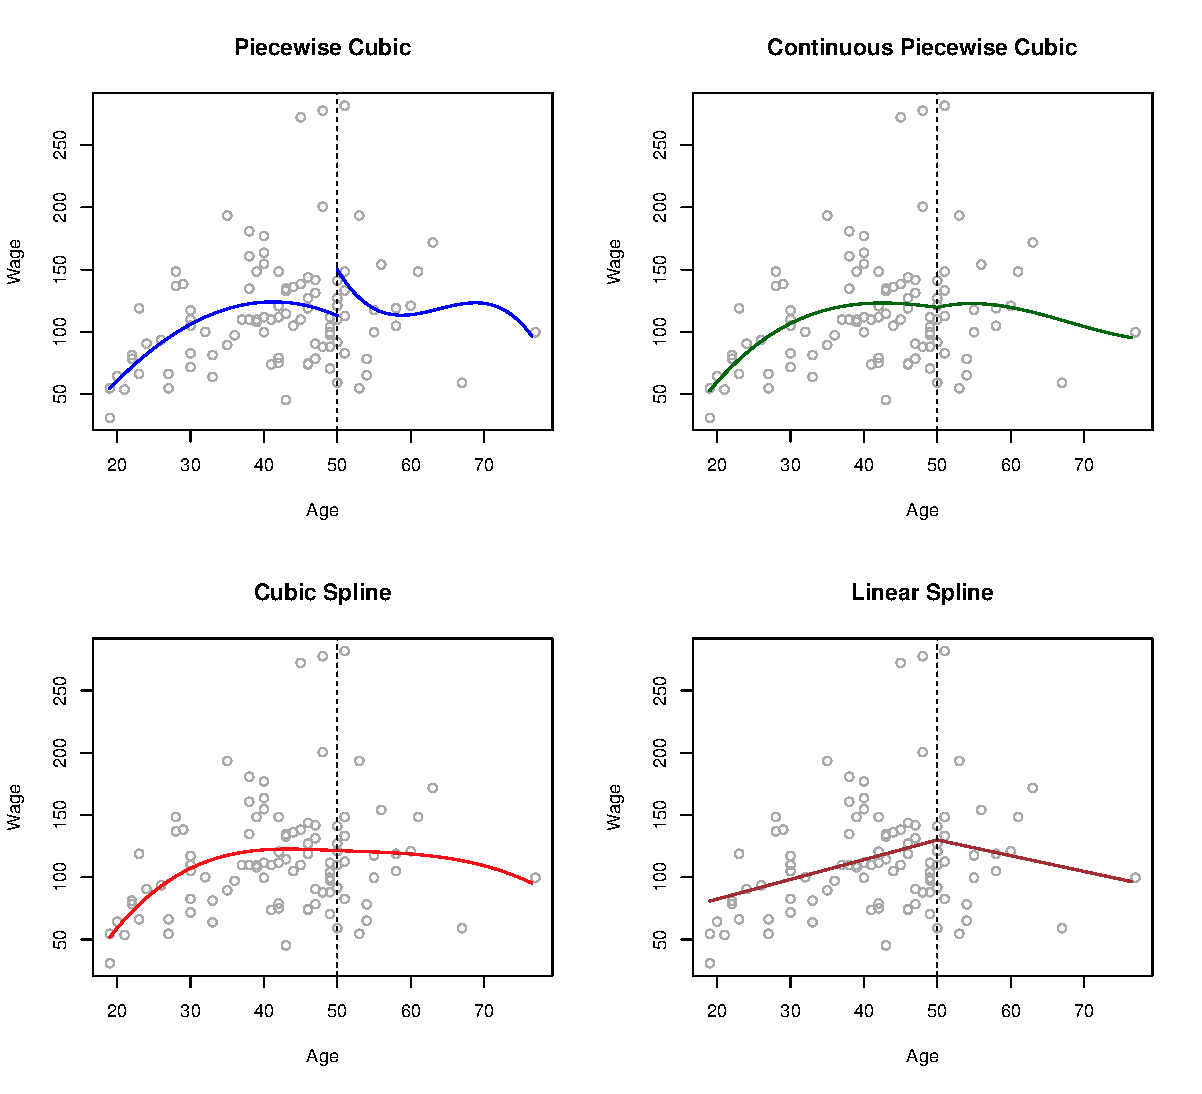
\includegraphics[width=0.99\textwidth]{7_3}
			\end{center}
		\end{column}
	\end{columns}
	\bl{Putting constraints on the knots of piecewise polynomials leads to splines.}
\end{frame}

\begin{frame}{Constraints and Splines}
	\begin{itemize}
		\item To construct a \e{cubic spline} we start from a piecewise polynomial
			of degree 3 and impose the following constraints.
			\begin{popblock}{0.4\textwidth}{}
				\begin{tabular}[h]{ll}
					{\bfseries\blue constraint} & {\bfseries\blue continuity} \\
					$b(x_i)$ & value \\
					$b'(x_i)$ & slope \\
					$b''(x_i)$ & curvature\\
				\end{tabular}
			\end{popblock}
		\item Each constraint frees up one degree of freedom.
		\item In general, cubic splines with $K$ knots use $K+4$ degrees of freedom.
	\end{itemize}
	\bl{We do not concern ourselves with the details involved in imposing the constraints.}
\end{frame}

\begin{frame}{Natural Splines}
	\vspace{-14mm}
	\begin{center}
		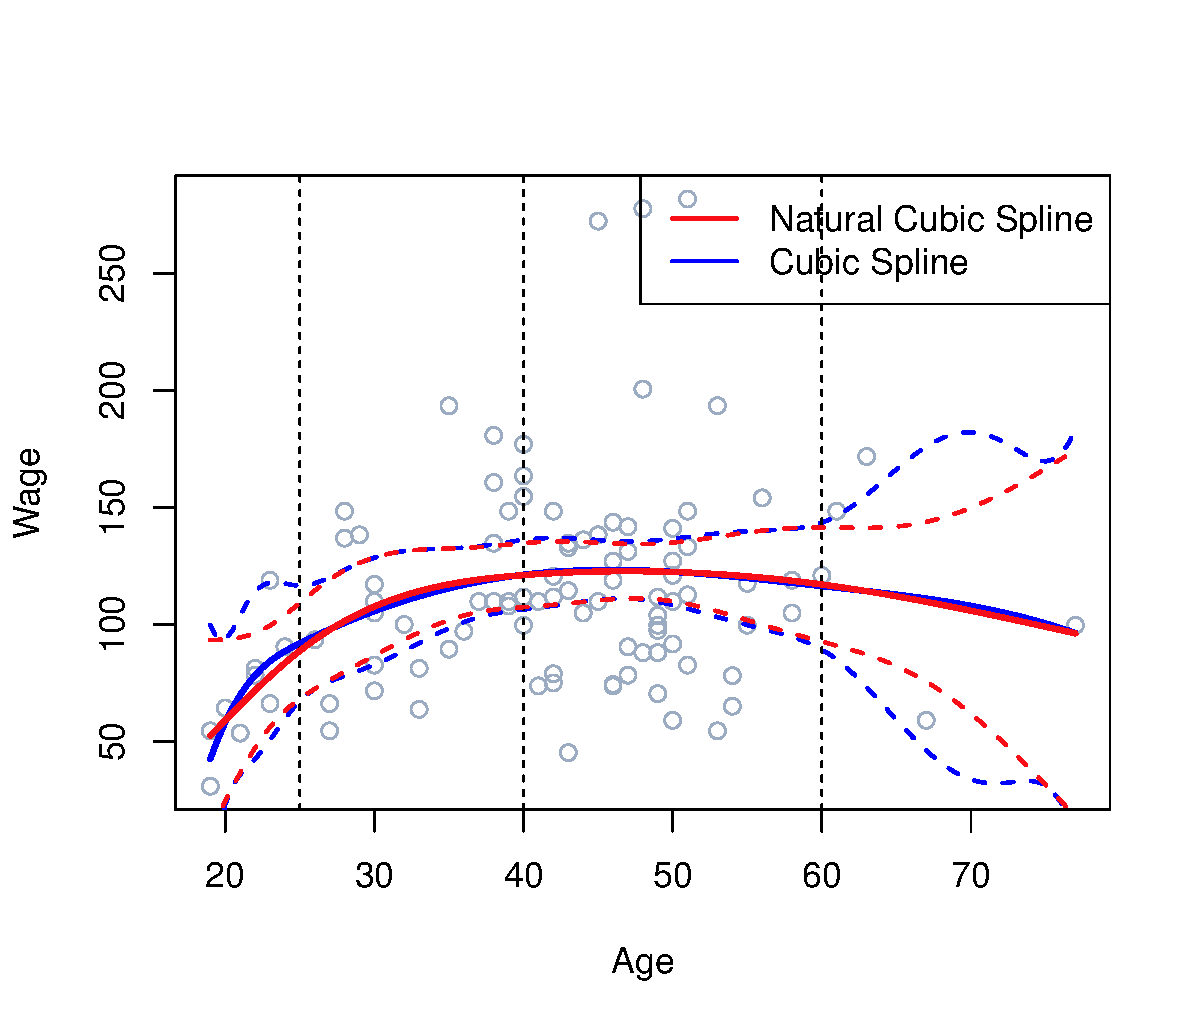
\includegraphics[width=0.6\textwidth]{7_4}
	\end{center}
	\vspace{-8mm}
	\begin{itemize}
		\item Splines can have large variance at the outer range of the predictors.
		\item \e{Natural splines} are constrained to be linear at the boundaries.
	\end{itemize}
	\bl{Note that the confidence interval for the natural spline is narrower.}
\end{frame}

\begin{frame}{Choosing $\bm{K}$ \& Knot Positions}
	\begin{center}
		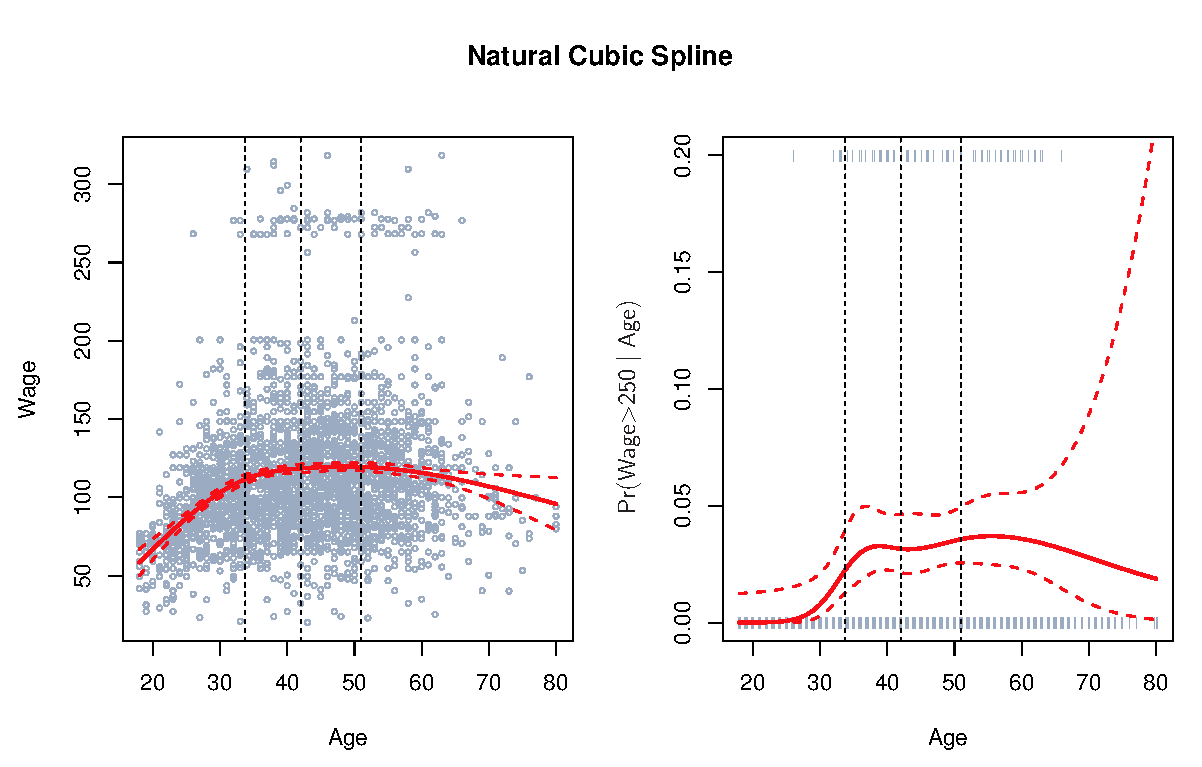
\includegraphics[width=0.7\textwidth]{7_5}
	\end{center}
	\bl{We usually specify the degrees of freedom and place the knots uniformly over quantiles .}
\end{frame}

\begin{frame}{Choosing $\bm{K}$ \& Knot Positions}
	\begin{center}
		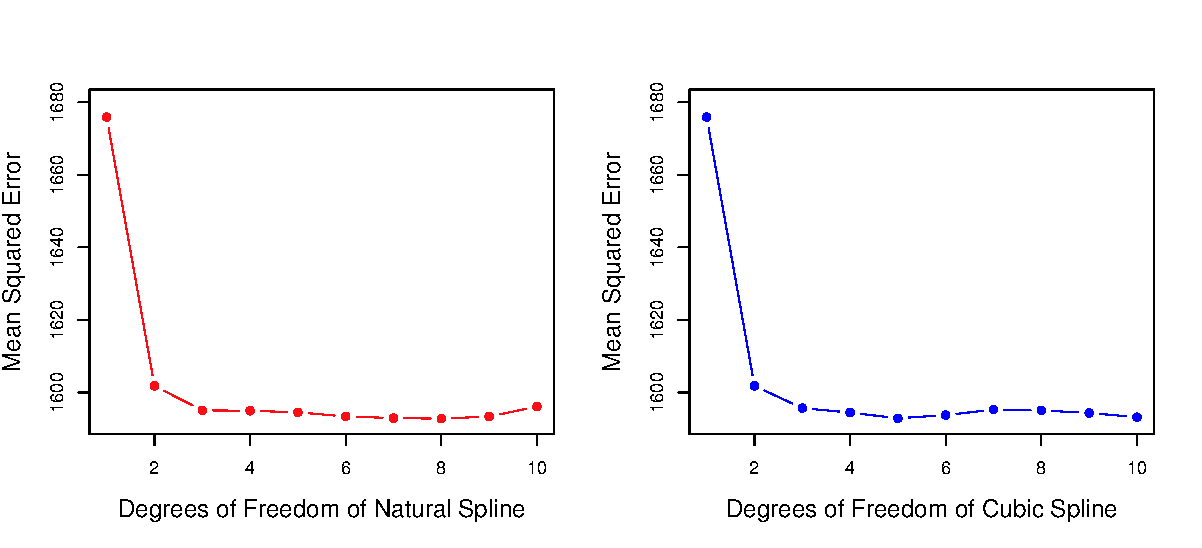
\includegraphics[width=0.9\textwidth]{7_6}
	\end{center}
	\bl{In practice -- you guessed it -- we use cross-validation.}
\end{frame}

\begin{frame}{Splines versus Polynomial Regression}
	\vspace{-8mm}
	\begin{center}
		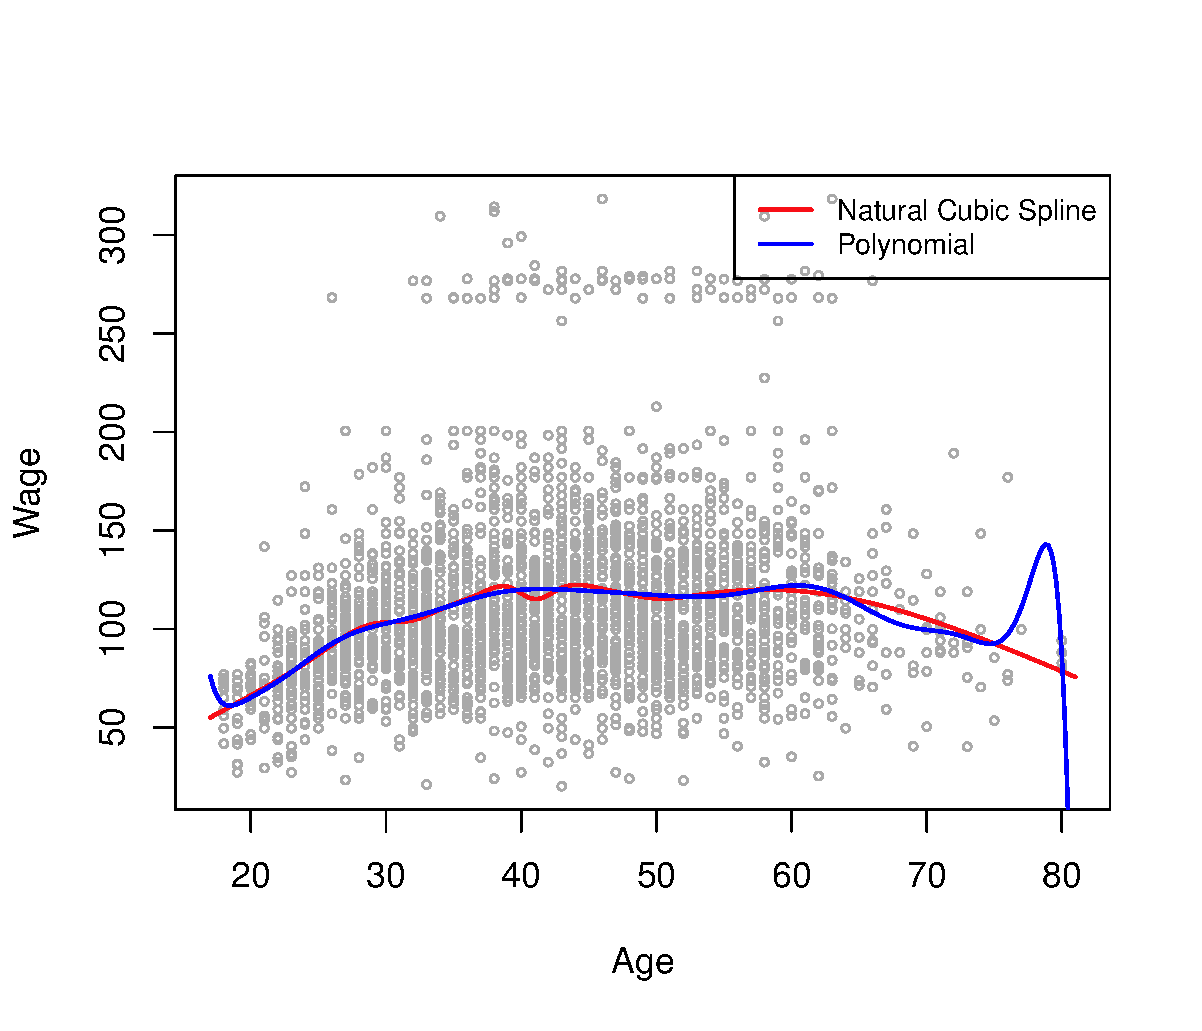
\includegraphics[width=0.6\textwidth]{7_7}
	\end{center}
	\vspace{-8mm}
	\bl{High degree polynomials tend to behave badly at the boundaries.}
\end{frame}

\begin{frame}{Smoothing Splines}
	\begin{itemize}
		\item \e{Smoothing splines} are a different approach to fitting splines.
		\item We want to find some \e{smooth} function $g(x)$ that fits the data well, that is
			\[
				\text{RSS} = \sum_{i=1}^n (y_i - g(x_i))^2
			\]
			is small.
		\item The smoothness can be imposes by minimising
			\[
				\underbrace{\sum_{i=1}^n (y_i - g(x_i))^2}_\text{loss} 
				+
				\underbrace{{\orange\lambda}\int g''(t)^2 dt}_\text{penalty}
			\]
	\end{itemize}
	\bl{The \e{loss + penalty} approach is very common in machine learning practice.}
\end{frame}

\begin{frame}{Choosing the $\bm{\lambda}$ Parameter}
	\vspace{-8mm}
	\begin{center}
		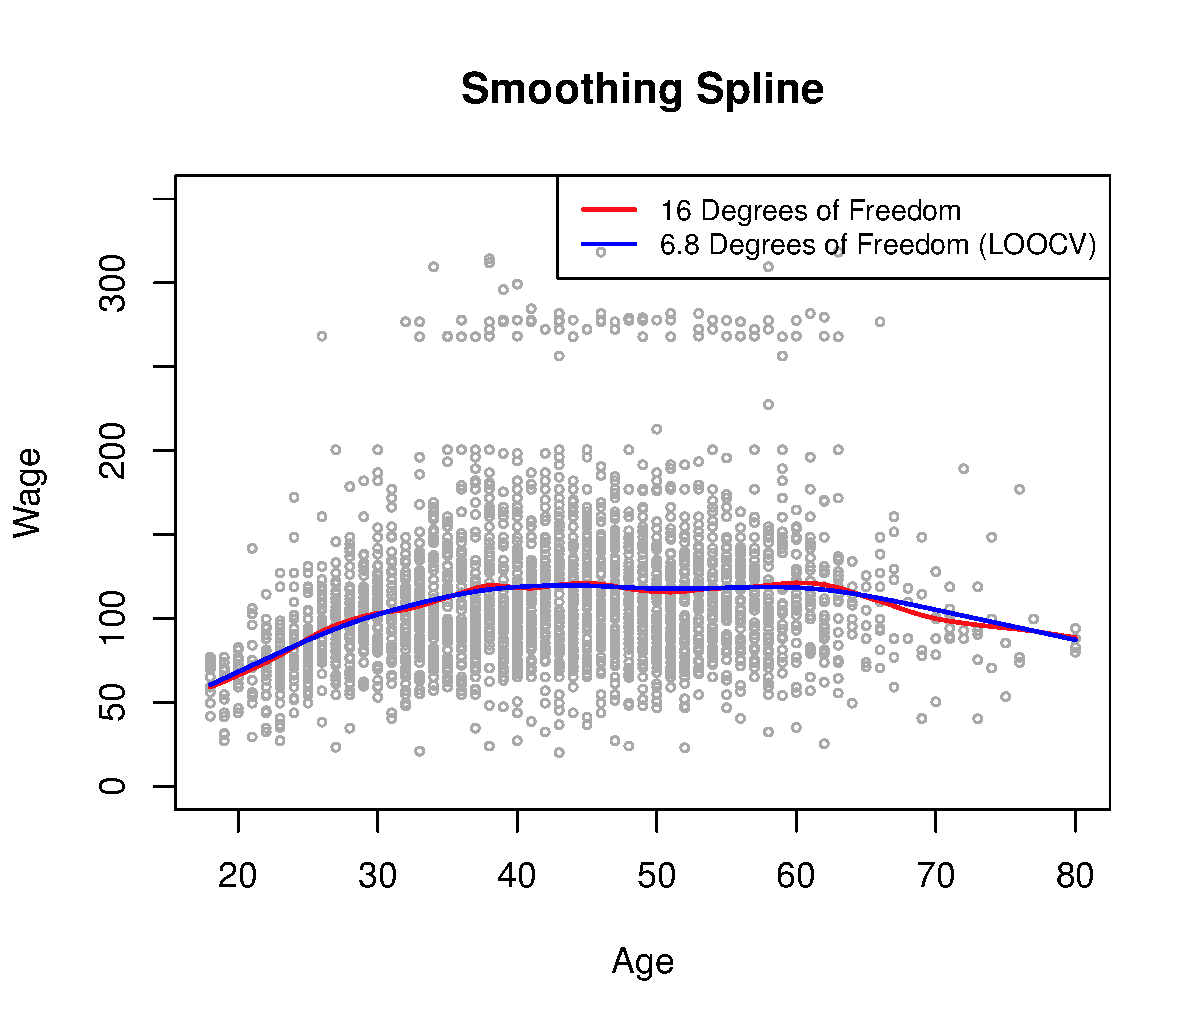
\includegraphics[width=0.6\textwidth]{7_8}
	\end{center}
	\vspace{-8mm}
	\bl{The $\bm{\lambda}$ parameter is continuous, leading to the concept of \e{effective degrees of freedom}.}
\end{frame}

\begin{frame}{Generalised Additive Models}
	\begin{itemize}
		\item We now release the condition of having a single predictor in the model.
		\item This leads to the concept of \e{generalised additive models} (GAMs).
		\item This is analogous of moving from simple linear regression to multiple
			linear regression.
		\item That is, the models can now take the form
			\begin{align*}
				y_i &= \beta_0 + \sum_{j=1}^p f_i(x_{ij}) + \epsilon_i\\
				{} &= \beta_0 +  f_1(x_{i1}) + f_2(x_{i2})
				+ \dots + f_p(x_{ip}) + \epsilon_i\\
			\end{align*}
			with \e{smooth} functions $f_j$.
	\end{itemize}
	\bl{The model still \e{additive} because we \e{add} separate $\bm{f_j}$ for each $\bm{X_j}$.}
\end{frame}

\begin{frame}{Generalised Additive Models}
	\begin{center}
		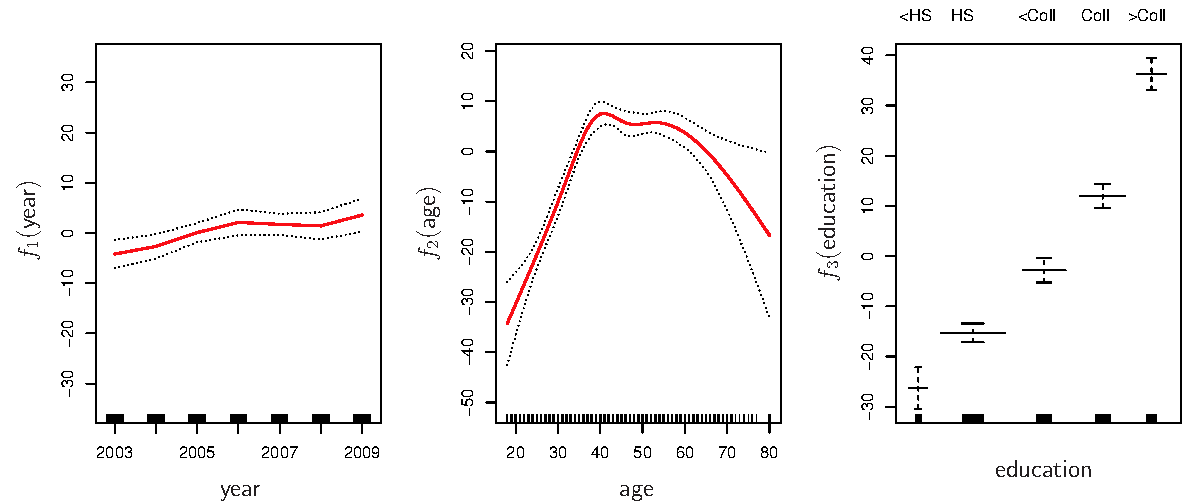
\includegraphics[width=0.8\textwidth]{7_11}
	
		\[
			\mdat{wage} = \beta_0 + f_1(\mdat{year}) + f_2(\mdat{age}) + f_3(\mdat{education}) 
			+ \epsilon
		\]
	\end{center}
	\bl{A GAM model on the Wage data set with two cubic splines and a qualitative variable.}
\end{frame}

\begin{frame}{Generalised Additive Models}
	\begin{center}
		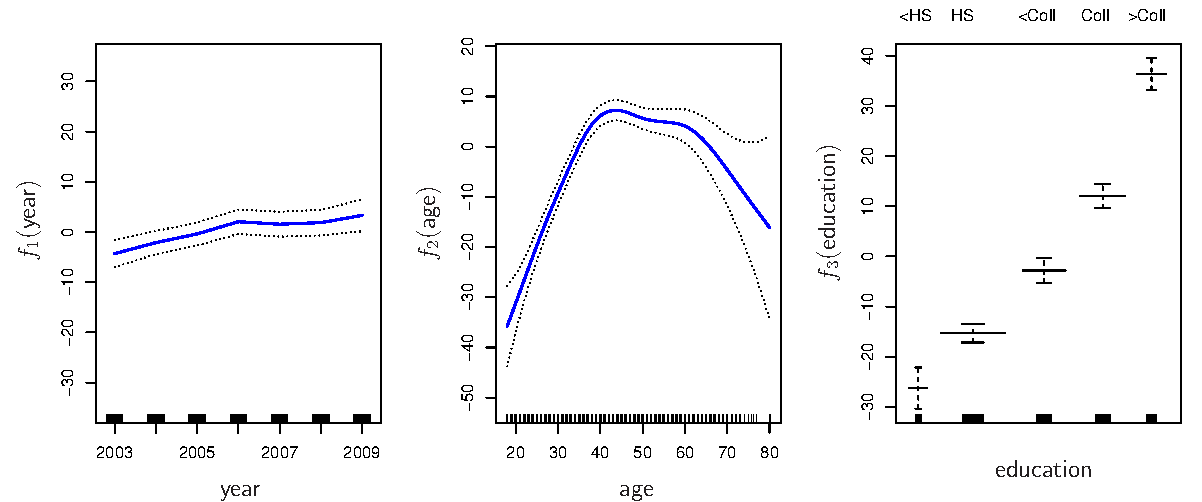
\includegraphics[width=0.8\textwidth]{7_12}
	
		\[
			\mdat{wage} = \beta_0 + f_1(\mdat{year}) + f_2(\mdat{age}) + f_3(\mdat{education}) 
			+ \epsilon
		\]
	\end{center}
	\bl{A GAM model on the Wage data set with two smoothing splines and a qualitative variable.}
\end{frame}

\begin{frame}{GAMs for Classification}
	\begin{itemize}
		\item GAMs can also be used for classification.
		\item Just like with ordinary linear models, we use logistic regression in this scenario:
			\[
				\log
				\left(
					\frac{p(X)}{1 - p(X)}
				\right) =
					\beta_0  + f_1(x_{i1}) + f_2(x_{i2})
					+ \dots + f_p(x_{ip}) + \epsilon_i
			\]
		\item For example:
			\[
				\log
				\left(
					\frac{p(X)}{1 - p(X)}
				\right) =
				\beta_0  + \beta_1\times\mdat{year} + f_2(\mdat{age})
				+ f_3(\mdat{education})
			\]
			where
			\[
				p(X) = P(\mdat{wage} > 250\vert\mdat{year}, \mdat{age}, \mdat{education}) 
			\]
	\end{itemize}
	\bl{That is, we want to predict whether the yearly income is greater than \$250,000.}
\end{frame}

\begin{frame}{GAMs for Classification}
	\begin{center}
		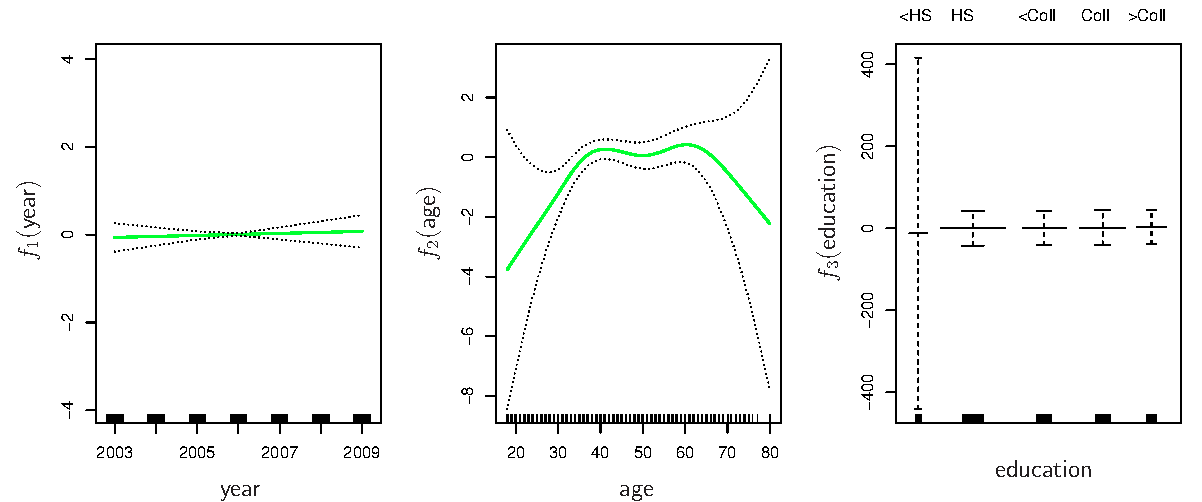
\includegraphics[width=0.8\textwidth]{7_13}
	
		\[
			p(X) = P(\mdat{wage} > 250\vert\mdat{year}, \mdat{age}, \mdat{education}) 
		\]
	\end{center}
	\bl{There seems to be a problem with the qualitative variable.}
\end{frame}

\begin{frame}{GAMs for Classification}
	\begin{center}
		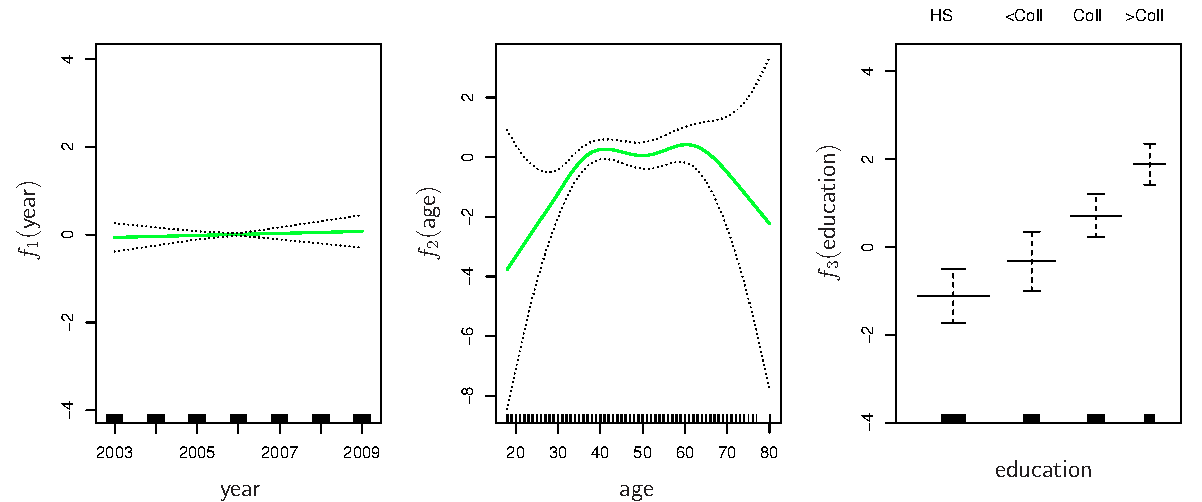
\includegraphics[width=0.8\textwidth]{7_14}
	
		\[
			p(X) = P(\mdat{wage} > 250\vert\mdat{year}, \mdat{age}, \mdat{education}) 
		\]
	\end{center}
	\bl{It turns out high school drop-outs never earn more than \$250,000/year.}
\end{frame}

\end{document}
